\documentclass[authoryear,12pt]{elsarticle}
\bibliographystyle{model2-names}
\usepackage{geometry}                % See geometry.pdf to learn the layout options. There are lots.
\geometry{letterpaper}                   % ... or a4paper or a5paper or ... 
%\geometry{landscape}                % Activate for for rotated page geometry
%\usepackage[parfill]{parskip}    % Activate to begin paragraphs with an empty line rather than an indent
\usepackage{graphicx}
\usepackage{amssymb}
\usepackage{amstext}
\usepackage{epstopdf}
\usepackage{ulem}
\usepackage{url}
\usepackage{natbib}

\usepackage{wrapfig}
\usepackage{subfig}

\textwidth 6in
\textheight 9in

\graphicspath{{images/}}

\DeclareGraphicsRule{.tif}{png}{.png}{`convert #1 `dirname #1`/`basename #1 .tif`.png}

%\title{Flying \xout{On} Empty}
\title{Graphical Exploration of the Deep-Water Horizon Oil Spill}
\author{Lendie Follett, Ulrike Genschel, Heike Hofmann\\Department of Statistics\\Iowa State University}
\date{\today}                                           % Activate to display a given date or no date

\begin{document}
\maketitle
%\tableofcontents
\begin{abstract}
Graphical exploration of the immediate impact of the Deep Water Horizon Oil Spill of 2010. 
\end{abstract}
\section{Introduction}
April 20th, 2010 marked the beginning of the largest oil spill in the history of off-shore drilling.  Following an explosion in the Deep-Water Horizon drilling rig and failure of all emergency systems, crude oil began to gush into the ocean.  After an estimated 4.9 million barrels of oil spilled into the sea, the leak was finally stopped on July 15th of 2010 when the well head was capped.  The completion of the relief well took until September 19, 2010.  The immediate impact of the oil spill on people and wildlife alike was overwhelming and can still be felt.  The oil destroyed many habitats for birds, turtles, and other marine wildlife.  Waters had to be closed for fishing, affecting the livelihood of the people that depended on the fishing industry. Longterm effects are certain. It is of course impossible to do an analysis that can reflect the breadth and complexity of the effects of the oil spill.  However, based on data provided by government sources we want to graphically demonstrate the immediate impact of the spill on wildlife, measured salinity - which has a major influence in determining oceanic flow, and environmental pollution through chemicals found in oil, in particular Polycyclic Aromatic Hydrocarbons (PAHs). 

% structure of the paper

%
\section{Graphical Exploration}
\subsection{Animal Sightings}
\begin{table}
\begin{tabular}[hbt]{lp{11cm}}\hline
\bf Variable & \bf Description \\\hline
Class & type of animal found: \\
& {\small Birds (5,552),   Whales and Dolphins  (98),  Sea Turtles (546)}\\
Species & species of animal \\
Latitude & latitude in degrees  \\
Longitude & longitude in degrees\\
Alive & condition of animal: \\
& {\small Alive (2,197), Dead (6,196)} \\
Observation Date & date of observation `mm-dd-yyyy'. \\\hline
\end{tabular}
\caption{Animal Sightings between April 26, 2010 and October 18, 2010, source: Avian Observations from US Fish and Wildlife (Southeast Region),  Marine Mammal Observations reported by  the National Marine Sanctuary, NOAA, and the Office of Protected Resources, NOAA.}
\label{table-animal}
\end{table}
\begin{figure}[htbp] %  figure placement: here, top, bottom, or page
   \centering
   \includegraphics[width=4in]{animal_deaths.png} 
   \caption{Satellite map of a part of the Gulf of Mexico. The location of the Deep Water Horizon rig is marked by a white cross. Each dot on top of the map represents the sighting of one dead animal: 5,552  birds (orange), 546 sea turtles (yellow), and 98 dolphins and whales (red). }
   \label{deaths}
\end{figure}
One of the visually most impressive and very emotional effects of any oil spill might be the pictures of oiled beaches littered with the washed-up bodies of oil-blackened animals. Incidentally, this was the motive of this year's winning entry in the Veolia Environment Wildlife Photographer of the Year by \citet{photo}

Counts for animal sightings, both alive and dead, are collected by the local Departments of Natural Resources and National Agencies. For the Data Expo 2011 Challenge we had access to data from the National Marine Sanctuary, the Office of Protected Resources as well as the US Bureau of Fish and Wildlife Service. Table \ref{table-animal} gives a more detailed overview of the variables that we used for our graphical exploration. 

Figure \ref{deaths} shows a satellite map, overlaid by a scatterplot indicating locations of animal sightings. Most of the sightings follow the coastline - which is not surprising, since that is where we have the easiest access to make these kind of observations. 

%This already points us to several problems with an interpretation of the data:
%% could we re-frame this in terms of missing data:
%% - we're missing data from the time before the oil spill
%% - missing frequency of observers: number of records should be (somewhat) related to # of observers. 
%%       some areas are more accessible to human observation than others
%%       immediately after the oil spill general public much more interested 
%% - location is recorded, but we need to be careful with interpretation
%
%firstly, the data is purely observational - records are only available since the start of the oil spill, but not from before, reducing our conclusions to a qualitative nature. An additional  complication is the selection bias that we are facing: some of the areas presumably impacted by the oil spill are less accessible to observation than others. % resulting in .
%  Furthermore, locations of dead animals sightings are affected by  currents. It would be very wrong to interpret beaches as particularly dangerous because of the high number of sightings of dead animals. Instead, we should draw comparisons on a larger scale by comparing coastal regions and use  the number  of dead animals as an indicator of the effect on a particular region.  We have to be aware that we are also dealing with a large percentage of unknowns: an unknown number of animals will have decayed or sunk to the seabed before being washed up on the beach, thereby going unnoticed and unreported.
%
%With those caveats in mind, we can still tell from the satellite map in Figure \ref{deaths} that 

The highest concentration of dead animals were found along the shores of Louisiana and Mississippi, closest to the oil rig. Each of the orange dots corresponds to one dead bird, yellow dots indicate dead sea turtle sightings, and red dots indicate large mammals, such as whales and dolphins. Overall a total of 6,196 animals were reported dead during a six month period.

\begin{figure}[htbp] %  figure placement: here, top, bottom, or page
   \centering
   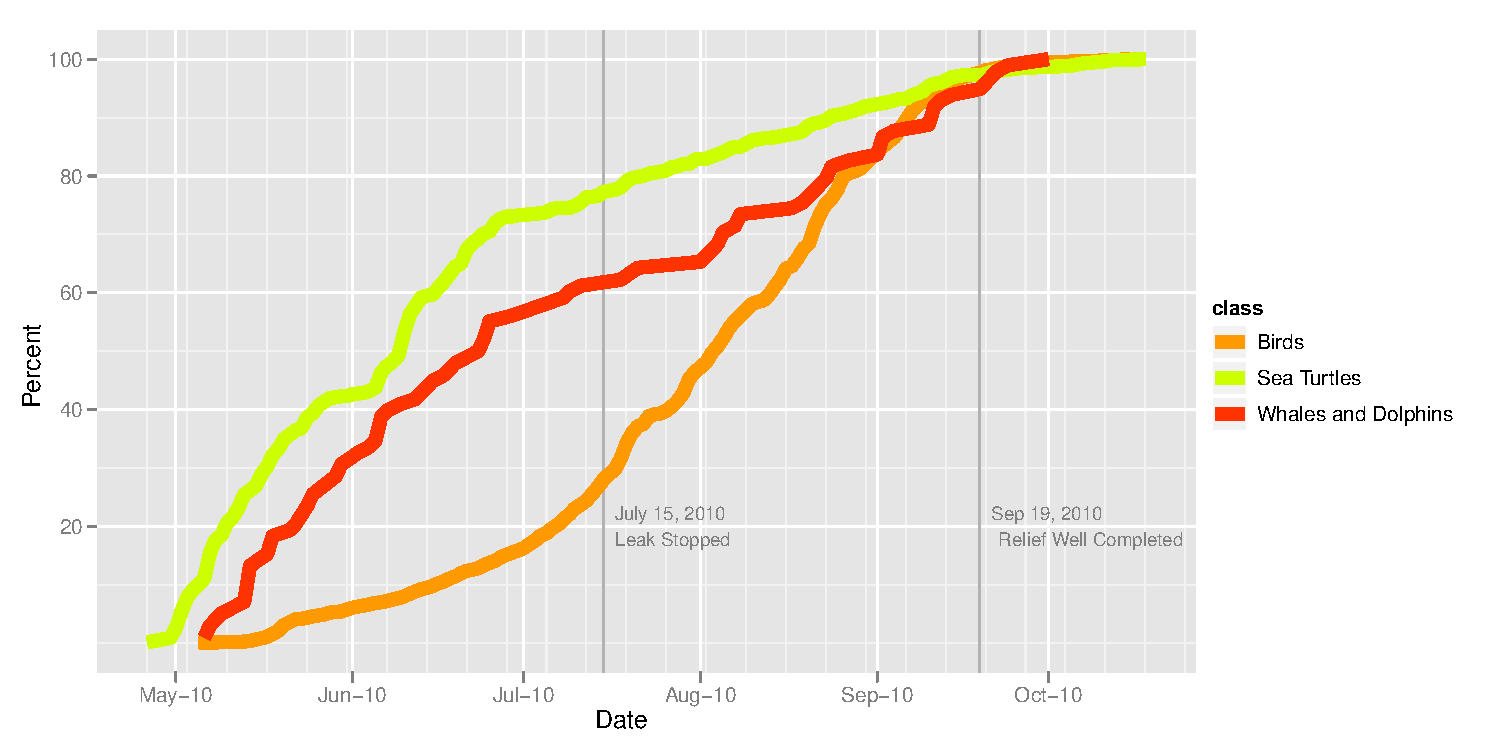
\includegraphics[height=1.75in]{death-rates.pdf} 
    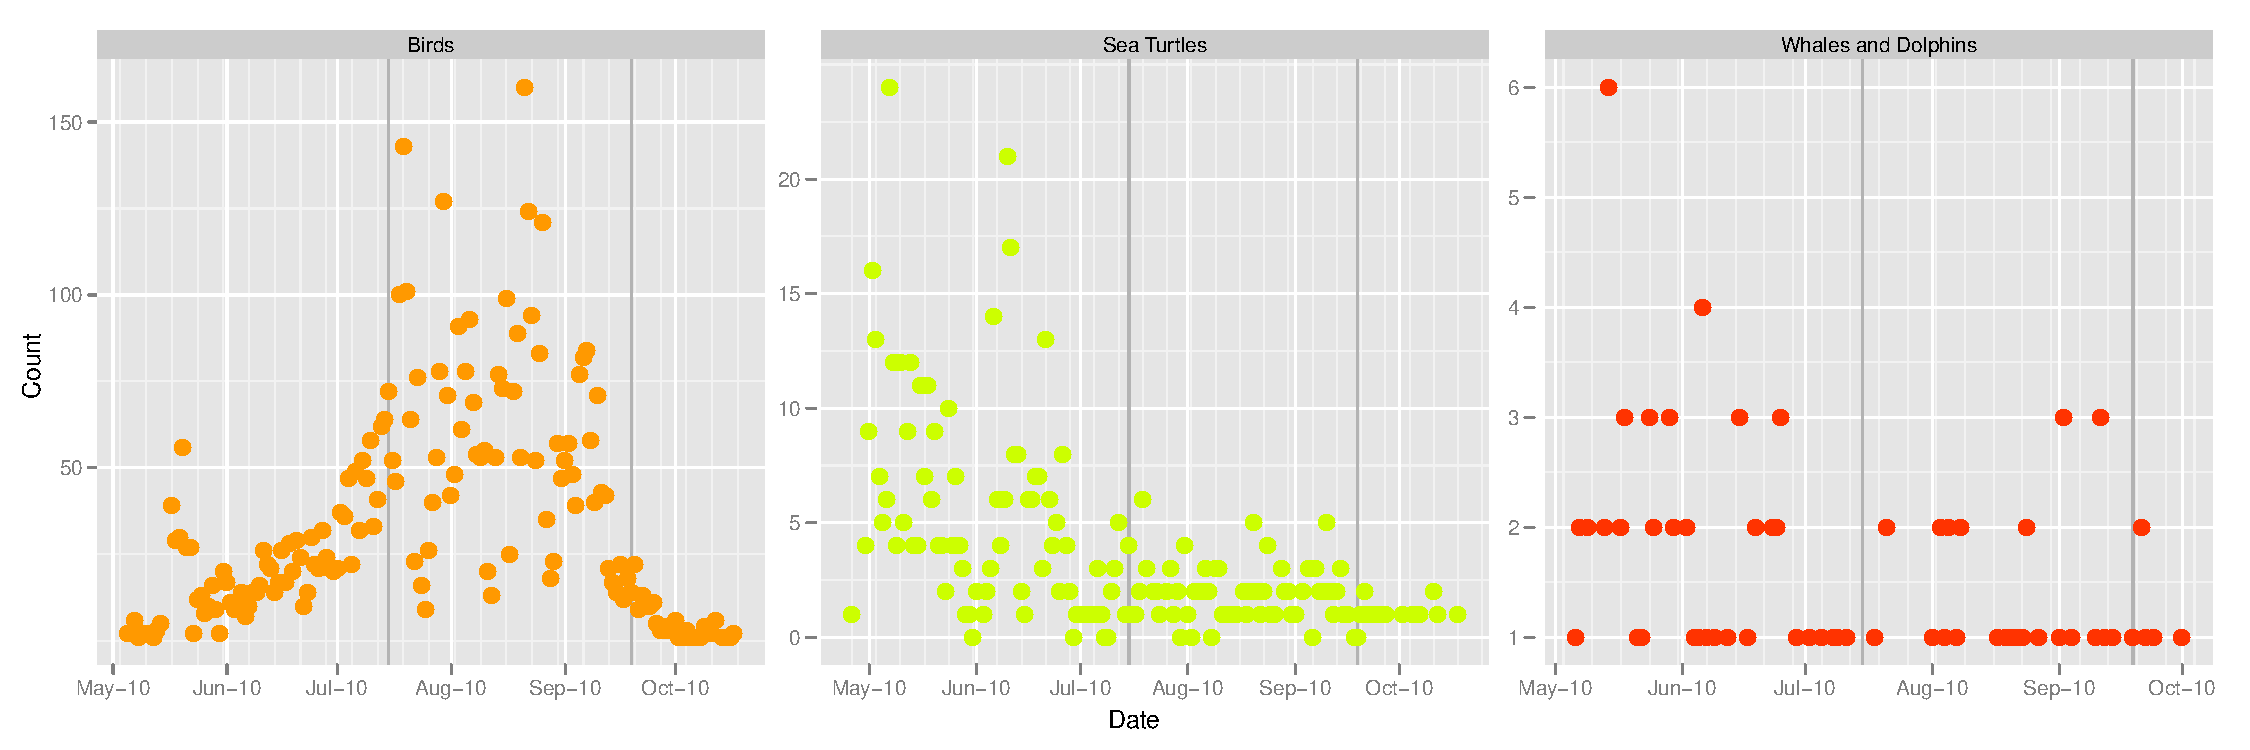
\includegraphics[height=1.75in]{daily-death-counts.pdf}
   \caption{Cumulative animal death rates by class  (top) and absolute number of dead animal sightings (bottom) between April and October 2010.\newline}
   \label{death rates}
\end{figure}


Birds, sea turtles, and dolphins and whales had unique death patterns during the data collection period as Figure \ref{death rates}  illustrates. The figure at the top shows a cumulative death rate for each species over time. Birds responded later to the disaster than sea turtles, whales and dolphins. They had a relatively low death rate from May to July, after which the rate began to increase. Sea turtles and dolphins and whales, on the other hand, had the highest death rates from May to July and from there it began to flatten out. \\
These patterns are shown in more detail in  the charts at the bottom of figure \ref{death rates}, which show daily death counts between May and October for each class of animals. For sea turtles, dolphins, and whales, the highest daily death counts occurred in the earlier weeks and then decreased over time.  The majority of dead bird findings occurred later in time and their death counts per day began to climb rapidly around July. After the leak was stopped, on July 15th, the number of daily deaths shows a high variability until it begins to decrease by mid-September. For sea turtles, also, stopping the leak seems to have the most profound impact on reducing the daily death counts. 

\begin{figure}[htbp] %  figure placement: here, top, bottom, or page
   \centering
   \includegraphics[width=6in]{turtles.png} 
   \caption{Four species of endangered or critically endangered sea turtles observed in the Gulf of Mexico from April 26th to October 18th 2010.  Blue dots indicate turtles found alive; red dots indicate those found dead.}
   % series of maps of 
   \label{turtles}
\end{figure}

Four species of sea turtles were found and identified during the data collection period, all of which are considered to be either threatened or endangered. These species are: Kemp's Ridley, Hawksbill Sea Turtle, Green Sea Turtle, and Loggerhead Sea Turtle. Figure \ref{turtles} shows when and where these turtles were found and whether they were living or dead. Most dead turtles, of all species, were found along the shoreline. Alive sea turtles were mostly spotted off the coast. There are, in particular, two main areas along the coasts of Louisiana and Florida in which the bulk of live sea turtles were found.  This is most evident among the Green Sea Turtle and Kemp's Ridley. The species with the greatest number of casualties found was Kemp's Ridley, an endangered species which lives primarily in the Gulf of Mexico.  It is more common for Kemp's Ridley sea turtles to be present in the northern part of the Gulf of Mexico during June, July, and August. Female Kemp's Ridleys, like other sea turtles, nest between May and July and lay their eggs on various beaches of the Gulf of Mexico  \citet{turtles}. From this information, we can understand that there were more turtles in the area during the months after the oil spill occurred, and thus more sea turtles to be found.  After August, however, it would be natural for these turtles to begin to leave the area and head south. Very few turtles were found after September.

\subsection{Chemicals}

\begin{table}
\begin{tabular}{lp{9.5cm}}\hline
\bf Variable & \bf Description \\\hline
Substance & Polycyclic Aromatic Hydrocarbon (PAH) substance \\
Date & date of observation.\\
Latitude & latitude in degrees. \\
Longitude & longitude in degrees. \\
Result &  measured amount \\
Unit &  unit of measurement: \\
& {\small ug/L for water, ug/k for sediment} \\
Danger Level* &  health effects:\\
& {\small carcinogenic (23,201), other health effects (3,640)} \\
Alkylation Multiplier** & used for calculations, see appendix A \\
Acute Potency Divisor** & used for calculations\\
Chronic Potency Divisor** & used for calculations \\\hline
\end{tabular}
\label{table.chemicals}
\caption{Water and sediment chemistry data of petrochemical products, sampled near the coastline in the months after the oil spill, source: US Environmental  Protection Agency.\newline
{\small *according to recommendations of \citet{pah-danger}}\newline
{\small **following \citet{pah-benchmark}} }
\end{table}



Various chemicals were sampled in the Gulf of Mexico during the months following the oil spill. This analysis focuses on Polycyclic Aromatic Hydrocarbons firstly because of their direct relationship with oil and secondly because of their toxicity to wildlife. Polycyclic Aromatic Hydrocarbons, or PAHs, are semi-volatile organic substances which come mainly from oil and the burning of oil. However, they can also come from exhaust and from the burning of gas, coal, garbage and other organic substances \citep{pah}.   Many of these substances are considered carcinogenic, mutagenic, and teratogenic and all are considered harmful to the health of living organisms. Based on EPA guidelines \citep{pah},  this information  was added to the given data. \\
Additionally, it was necessary to put the measurements into a more interpretable form in order to judge the effect of these chemicals on life in the Gulf of Mexico.
 We followed the approach by \citet{pah-benchmark}: measurements of the PAHs are aggregated for each location and considered in terms of their acute and chronic potency: a location is considered to be  at a chronic level when the amount of harmful substances is thought to bring harmful effects over a long period of time. For an acute level the overall amount of substances is at a level that rapidly induces a negative and possible irreversible effect in an organism. 
 
Each PAH substance has a unique  threshold at which it has an acute or chronic effect on humans. These thresholds are called potency divisors, which are in turn  used to find corresponding potency ratios by -- essentially -- dividing the observed amount by its divisor (for a more detailed discussion, please see appendix \ref{benchmarks}). An acute ratio of 1 can be interpreted as the amount of a substance that is considered to be harmful.

For surface water and sediment samples alike, these ratios are additive in effect. We can therefore sum ratios at each location to determine the overall effect of all chemicals on human beings. Again, a ratio of greater than 1 on the acute level can be considered as immediately causing harmful effects on human beings.


\begin{figure}[htbp] %  figure placement: here, top, bottom, or page
   \centering
   \includegraphics[width=5in]{acute-timeline3.png} 
   \caption{Timeline of logarithm of acute potency ratios.  Points are colored according to a substance's effect on health. There is a period of time between June and July in which the acute value is heightened.  Points which exceed the acute benchmark are labeled.}
   \label{pah-timeline}
\end{figure}


Figure \ref {pah-timeline} shows the (log) acute potency ratios  for measurements recorded between May and August of 2010. Three measurements of PAH substances exceed the acute potency ratio, indicating that these substances by themselves were high enough to be acutely dangerous. All of them belong to the Chrysene family, which  is considered to be carcinogenic. During the  period between June and July  measurements of these PAH substance showed elevated values.

\begin{figure}[htbp] %  figure placement: here, top, bottom, or page
   \centering
   \includegraphics[width=3.5in]{chron-acute-map.png} 
   \caption{Satellite map of the Gulf Coast area overlaid by locations at which PAH measurements were taken (light blue dots). Yellow dots represent locations that are at a chronic level, red dots mark locations with an acute level.  The most dangerous area is along the outermost shore of Louisiana: many locations here have PAH levels at or above chronic or acute benchmarks.}
   \label{pah-map}
\end{figure}


Figure \ref{pah-map} shows a map of the gulf coast overlaid by light blue points at locations where PAH measurements were taken. Locations with elevated PAH values are emphasized by colored dots: yellow (at or above chronic) and red (at or above acute thresholds).  Particularly along the outer coast of Louisiana, many of the observed PAH values exceeded the benchmarks.  This might be an indication, that this area had the most direct contact with the oil.  

\subsection{Salinity}

\begin{table}
\begin{tabular}{lp{9.5cm}}\hline
\bf Variable & \bf Description \\\hline
Date & date of observation. \\
Latitude & latitude in degrees \\
Longitude & longitude in degrees. \\
Depth & depth of measurement in feet \\
Salinity &  amount of salinity in mg/l \\
Type &  type of measuring device: \\
& {\small Boat (24,381), Float (10,332), Glider (368,563)} \\\hline
\end{tabular}
\label{table.salinity}
\caption{, source: NOAA}
\end{table}

Where does the oil go? - In the days after the explosion this was the second most interesting question after 'how big is the spill?'.  The oil flow is mostly driven by the current, which can be determined based on measurements of salinity, depth and temperature. 
In order to keep track of the oil movement, NOAA pulled most of its resources into the Gulf area to measure these characteristics:  2 boats, 11 floats, and 10 gliders, which recorded salinity, temperature, and depth measurements at various locations in the Gulf of Mexico. 
The floats tended to stay in the deeper water while the boats and the gliders recorded measurements in locations further away from the oil rig.  Figure \ref {Boats, Floats and Gliders} show the patterns of these three measuring methods. 

\begin{figure}[htbp] %  figure placement: here, top, bottom, or page
   \centering
   \includegraphics[width=3.5in]{boats-floats-gliders.png} 
   \caption{Paths of Boats, Floats, and Gliders. }
   \label{Boats, Floats and Gliders}
\end{figure}
Figure \ref {salinity-timeline} pictures  salinity measurements over the whole data collection period. Points are color coordinated by time to link left and right display. Approximately 99 \% of the salinity measurements stayed within a close range of values between 34 and 38 mg/l.
We deemed values of 34 mg/l as unusually low and highlighted their location in the right side of figure \ref{salinity-timeline}. The highest concentration of these points is found near the rig during June and July.
\begin{figure}[htbp] %  figure placement: here, top, bottom, or page
   \centering
   \includegraphics[width=2.8in]{salinity-time.png} 
   \includegraphics[width=2.8in]{salinity-map.png} 
   \caption{Salinity measurements: over time (left) and by location (right)> Salinity measurements only rarely fall below 34 mg/l. In the months after the start of the oil spill salinity frequently drops below 34 mg/l. For later weeks this happens in particular in locations close to the oil rig.}
   \label{salinity-timeline}
\end{figure}

\begin{figure}[htbp] %  figure placement: here, top, bottom, or page
   \centering
   \includegraphics[width=4in]{salinity-depth.jpeg} 
   \caption{Relationship between depth and salinity grouped by each unique latitude and longitude combination. Depth and salinity almost always maintain a fixed relationship, as seen in most of the observations. However, some areas, mainly those at the surface of the water, experienced unusually low values of salinity. Two areas, which were measured by a boat, had a depth-salinity relationship very unlike the rest.}
   \label{Depth-Salinity}
\end{figure}
Depth and salinity form a close relationship as can be seen in Figure \ref {Depth-Salinity}. For depths beyond 100 feet salinity levels are nearly constant. This is violated for  many measurements taken near the surface. Figure \ref {Depth-Salinity}  also shows  two lines of measurements taken by a boat which do not follow the normal relationship. The surface water measurement was far below normal observations and from there salinity dropped rapidly with depth. This, however, was in locations far from the rig and might have been unrelated incidents.

\subsection{Tools used}
The tools that we used for formatting the data and making the charts are:
{\tt R} \citep{R2011}, {\tt ggplot2} \citep{ggplot2}, {\tt RgoogleMaps} \citep{RgoogleMaps}, link between {\tt ggplot2} and {\tt RgoogleMaps} provided by \citet{kahle2010} as part of his entry in the ggplot2 competition.



\section{Conclusions}

Although there is no doubt that the oil spill caused a tremendous amount of damage, the lack of data makes it difficult to draw conclusions. We have no information on the actual cause of death of the birds, sea turtles, dolphins, and whales.  We also do not have past data to compare these findings with and so we can only reasonably assume that this number of dead animals is unusual. 

It is also hard to make definite inferences based on the PAH measurements.  While we know PAH substances were found at harmful levels along the coast, we do not have baseline data to compare post-spill levels to. As with the animal deaths, we can only reasonably assume that the high levels of PAHs are unusual for the area. 

Past data was available for salinity, however, the area in which these pre-spill salinity values were measured is quite different from the area in which the post-spill salinity values were measured.  Salinity measurements taken along the coastline will be quite different and therefore not directly comparable to those taken in the middle of the Gulf of Mexico. Better baseline data would have facilitated making conclusions about the effects of the Deep-Water Horizon oil spill on chemicals in the gulf, these chemicals' effects on wildlife, and salinity levels.

 What we do know is that the environmental conditions were highly unfavorable during the months after the oil spill. Polycyclic Aromatic Hydrocarbons were found at chronic and acute levels along the shoreline of the Gulf of Mexico. These levels are high enough to cause cancer and disrupt reproduction, development, and the immune system of organisms. Effects of these PAHs are likely to be felt long after the spill. Animals which did survive the initial spill and its aftermath such as birds, sea turtles, dolphins, and whales are all at risk of experiencing related health problems in the future. For this reason, the numbers in Figure 1, which only cover a 5 month period after the spill, do not entirely represent the number of animals that will have ultimately died as a result of the oil spill. The Deep-Water Horizon oil spill was a disaster which affected the environment, wildlife, and society upon impact, and will continue to do so for an indefinite number of years.

\begin{appendix}
\section{Benchmark Calculations}\label{benchmarks}
\subsection{Water Measurements}
Chronic and acute benchmark vales are computed based on the observed amount of PAH substance as follows:

\begin{eqnarray*}
\lefteqn{\text{Acute/Chronic Benchmark Value} =} \\
&&\sum \frac{\text{Alkylation Multiplier} \times \text{Measured Amount of Substance} (\mu g/L)}{\text{Acute/Chronic Potency Divisor}}
\end{eqnarray*}

\subsection{Sediment Measurements}
For substances measured in sediment, the amount of organic carbon for that area must additionally be used to find the acute and chronic potency ratios. Taking the organic carbon into consideration is important for sediment samples because, when it is present in the sediment, the PAHs bind to it, thus making the PAHs less toxic. Organic carbon, like any other substance, was measured at each location.

The following formulas show how we attained the chronic and acute benchmark values for sediment:
\begin{center} \textbf{Sediment} \end{center}

\begin{eqnarray*}
\lefteqn{\text{Acute/Chronic Benchmark Value} =} \\
&& \sum \frac{\text{Alkylation Multiplier} \times \frac{\text{Measured Amount of Substance} (\mu g/kg)}{\text{Organic Carbon}}}{\text{Acute/Chronic Potency Divisor}}
\end{eqnarray*}

\end{appendix}

\bibliography{references}



\end{document}  